\chapter{ENDPOINT VE SİSTEM GÜVENLİĞİ}

\section*{Giriş}
Endpoint güvenliği, modern siber güvenlik stratejilerinin temel taşlarından biridir. Bu bölümde endpoint koruma platformları, sistem güvenliği teknolojileri ve uç nokta güvenlik yönetimi konularını detaylı olarak inceleyeceğiz.

\section{Endpoint Protection Platform (EPP) Teknolojileri}

Endpoint Protection Platform (EPP), bir kuruluşun ağındaki uç noktaları (endpoint) siber tehditlere karşı korumak için tasarlanmış entegre bir güvenlik çözümüdür. Uç noktalar, dizüstü bilgisayarlar, masaüstü bilgisayarlar, sunucular, mobil cihazlar ve IoT cihazları gibi ağa bağlanan herhangi bir cihazı içerir. EPP'ler, geleneksel antivirüs yazılımlarının ötesine geçerek, çok katmanlı bir savunma yaklaşımı sunar. Bu çözümler, proaktif tehdit avlama, davranışsal analiz, makine öğrenimi ve istihbarat entegrasyonu gibi gelişmiş teknikler kullanarak bilinmeyen tehditleri tespit etme yeteneğine sahiptir. EPP'nin temel bileşenleri arasında gelişmiş antivirüs koruması, uygulama kontrolü, cihaz kontrolü ve veri kaybı önleme (DLP) yer almaktadır.

\subsection{Next-Generation Antivirus (NGAV) ve Machine Learning}

Geleneksel antivirüs (AV) çözümleri, bilinen tehditlere karşı bir imza veritabanını kullanarak çalışmaktadır. Bu model, yeni ve bilinmeyen tehditlerin ortaya çıkma hızı karşısında yetersiz kalmıştır. Bu yetersizlik, modern siber tehditlerin sürekli evrilen doğasına yanıt olarak Next-Generation Antivirus (NGAV) teknolojisinin geliştirilmesini tetiklemiştir. NGAV, geleneksel AV'nin imza tabanlı yaklaşımının aksine, makine öğrenmesi (ML), yapay zeka (AI), davranışsal tespit ve istismar önleme gibi ileri teknolojileri kullanarak bilinmeyen tehditleri dahi öngörmekte ve anında engellemektedir. Bu teknolojik değişim, güvenliğin sadece "bilinen kötüye karşı savunma"dan, "anormalin proaktif olarak tespiti"ne doğru evrildiğini göstermektedir.

NGAV'ın temel gücü, AI ve ML algoritmalarını kullanmasından kaynaklanmaktadır. Bu algoritmalar, dosya çalıştırılmadan önce milyonlarca dosya karakteristiğini gerçek zamanlı olarak analiz etmekte ve bir dosyanın kötü amaçlı olup olmadığını belirlemektedir. Bu imzasız teknoloji, hem bilinen hem de bilinmeyen kötü amaçlı yazılımları, uç nokta internete bağlı olmasa bile tespit etme ve engelleme yeteneği sunmaktadır. Ayrıca, NGAV çözümleri, dosyasız (fileless) saldırılar gibi geleneksel antivirüsleri atlatmak için tasarlanmış, sisteme yerleşik araçları (örneğin, PowerShell) kötüye kullanan tehditlere karşı da koruma sağlamaktadır. NGAV çözümleri, genellikle bulut tabanlı bir mimariyle çalıştığından, tek bir hafif ajan (lightweight agent) aracılığıyla uç noktalara dağıtılmakta ve sistem performansı üzerinde minimal etki yaratmaktadır. Bu bulut mimarisi, çözümün saatler içinde kurulmasına olanak tanırken, altyapı bakımı ve imza veritabanı güncelleme yükünü de ortadan kaldırmaktadır. NGAV, sadece daha iyi tespit yetenekleri sunmakla kalmayıp, aynı zamanda daha hızlı yanıt süreleri (MTTR) ve güvenlik personeli için daha az operasyonel yük sağlamaktadır.

\subsection{Behavioral Analysis ve Heuristic Detection}

Davranışsal analiz, bir sistemdeki kullanıcıların ve varlıkların normal aktivitelerini öğrenerek ve bu normal davranıştan sapmaları (anomalileri) tespit ederek çalışmaktadır. Bu yaklaşım, saldırganların geleneksel imza tabanlı sistemleri atlatmak için kullandığı yeni veya gizli yöntemlere karşı özellikle etkilidir. Sezgisel (heuristic) tespit ise, bilinen bir tehdit imzasıyla eşleşmeyen, ancak kötü amaçlı davranış kalıpları sergileyen kodları veya dosyaları proaktif olarak analiz etme yeteneğini ifade etmektedir. Bu iki teknik, özellikle sıfır-gün (zero-day) zafiyetlerini ve bilinmeyen tehditleri belirlemek için hayati öneme sahiptir.

Kullanıcı ve Varlık Davranış Analizi (UEBA), davranışsal analizin ileri bir formudur. UEBA, makine öğrenmesi algoritmalarını kullanarak kullanıcı ve varlık hareketlerinin temel bir modelini oluşturmaktadır. Bu sayede, güvenlik ekipleri anormal oturum açma girişimlerini, yetkisiz erişim denemelerini veya bir kullanıcının normalde erişmediği verilere ani erişimini daha erken aşamada tespit edebilmektedir. Bu durum, hem içeriden gelebilecek tehditlere hem de dış saldırganların kaba kuvvet veya diğer sinsi yöntemlerle sistemlere sızma girişimlerine karşı erken uyarı sağlamaktadır. Bir sistem, tek bir anomaliyi hemen kötü niyetli olarak işaretlemese de, bir saldırı döngüsü boyunca birden fazla anormal davranışın varlığı daha büyük bir riskin göstergesi olabilmektedir. Bu da güvenlik analistlerinin hangi uyarılara öncelik vermesi gerektiğini belirlemesine yardımcı olmaktadır. Sonuç olarak, davranışsal analiz ve UEBA, güvenlik analistlerine eyleme geçirilebilir içgörüler sunarak olaylara daha hızlı ve etkili bir şekilde yanıt verilmesini sağlamaktadır.

\subsection{Application Control ve Software Restriction Policies}

Uygulama kontrolü, bir sistemde hangi yazılımların çalışabileceğini yöneten bir siber güvenlik önlemidir. Bu önlemler, yetkisiz veya kötü amaçlı yazılımların çalıştırılmasını önleyerek güvenliği artırmayı amaçlamaktadır. Temel olarak iki ana strateji bulunmaktadır: \textbf{blacklisting (engellenenler listesi)} ve \textbf{whitelisting (izin verilenler listesi)}. Blacklisting, bilinen zararlı yazılımların çalışmasını engellerken, whitelisting yalnızca güvenilen ve onaylanmış uygulamaların çalışmasına izin vermektedir. Whitelisting, daha katı bir güvenlik duruşu sunmasına rağmen, yönetimi daha karmaşık olabilmektedir.

Windows ortamında, uygulama kontrolü için kullanılan çeşitli yerleşik mekanizmalar bulunmaktadır. Software Restriction Policies (SRP), Grup İlkesi tabanlı bir özellik olup, yazılımların dosya adı, hash değeri, yayıncısı veya dosya yolu gibi özelliklerine göre çalışmasını kontrol etmektedir. Ancak, Microsoft, Windows 10'un belirli sürümlerinden ve Windows Server 2019'dan itibaren SRP yerine daha modern ve gelişmiş olan \textbf{AppLocker} ve \textbf{Windows Defender Application Control (WDAC)} çözümlerini kullanmayı önermektedir.

WDAC, sanallaştırma tabanlı güvenlik (VBS) kullanarak çekirdek (kernel) seviyesindeki kodlar dahil olmak üzere, sistemde hangi uygulamaların çalışacağını kısıtlamaktadır. Bu sayede, kötü amaçlı komut dosyaları ve dosyasız saldırılar gibi modern tehditlere karşı daha güçlü bir koruma sağlanmaktadır. WDAC politikaları, PowerShell komutları veya Microsoft tarafından sağlanan özel bir sihirbaz aracılığıyla oluşturulabilmekte ve yönetimsel araçlarla (örneğin, GPO veya MEMCM) uç noktalara dağıtılabilmektedir.

\subsection{Pratik Yönergeler ve Komut Örnekleri}

Windows ortamında uygulama kontrolü politikalarını uygulamak için izlenebilecek adımlar ve örnek komutlar aşağıda sunulmuştur.

\begin{enumerate}
    \item \textbf{AppLocker ile Varsayılan Kural Oluşturma:}
    \begin{itemize}
        \item Bir yönetici hesabıyla Windows'a oturum açın ve \texttt{secpol.msc} komutunu çalıştırarak Yerel Güvenlik Politikası Düzenleyicisi'ni açın.
        \item \textbf{Application Control Policies} bölümünden \textbf{AppLocker}'a gidin.
        \item \textbf{Executable Rules} öğesine sağ tıklayarak \textbf{Create Default Rules} seçeneğini belirleyin. Bu işlem, yöneticilerin ve Program Files/Windows klasörlerindeki programların çalışmasına izin veren üç varsayılan kural oluşturacaktır.
    \end{itemize}
    \item \textbf{Belirli Bir Uygulamayı Engellemek İçin Kural Oluşturma (Yayıncı Kuralı):}
    \begin{itemize}
        \item Aynı konsolda \textbf{Executable Rules} öğesine sağ tıklayın ve \textbf{Create New Rule} seçeneğini seçin.
        \item İzin türü olarak \textbf{Deny}'ı seçin ve sonraki adımda ana koşul olarak \textbf{Publisher}'ı belirleyin.
        \item \textbf{Browse} düğmesine tıklayarak engellemek istediğiniz \\
        uygulamanın (\texttt{.exe}) dosyasını seçin. Örneğin, \texttt{chrome.exe}.
        \item Yayıncı (Publisher) bilgileri otomatik olarak doldurulacaktır. Kuralı tüm Chrome sürümlerine uygulamak için kaydırıcıyı \textbf{File name} seviyesine getirin ve kuralı kaydedin. Bu kural, Google Chrome'un tüm sürümlerinin çalışmasını engelleyecektir.
    \end{itemize}
    \item \textbf{WDAC Politikası Oluşturma ve Dönüştürme:}
    \begin{itemize}
        \item WDAC Wizard'ı kullanarak bir XML politikası oluşturun.
        \item Yönetici haklarıyla PowerShell ISE'yi açın ve oluşturulan XML politikasını dağıtılabilir ikili (.p7b) formata dönüştürmek için aşağıdaki komutu çalıştırın:
        \begin{verbatim}
ConvertFrom-CIPolicy -XmlFilePath "C:\wdac\policy.xml" 
    -BinaryFilePath "C:\wdac\siPolicy.p7b"
        \end{verbatim}
    \end{itemize}
\end{enumerate}

\subsection{Device Control ve Removable Media Protection}

Cihaz kontrolü ve taşınabilir medya koruması, organizasyonun güvenliğini artırmak ve veri sızıntısını önlemek için kritik önlemlerdir. Bu stratejiler, USB bellekler, harici diskler, CD/DVD'ler gibi taşınabilir medya cihazlarının uç noktalarda kullanımını düzenlemeyi ve izlemeyi amaçlamaktadır. Bu kontroller, kötü amaçlı yazılımların bu cihazlar aracılığıyla sisteme sızmasını engellediği gibi, hassas verilerin yetkisiz bir şekilde dışarıya aktarılmasının da önüne geçmektedir.

Windows ortamında, cihaz kontrolü genellikle Grup İlkesi Yönetimi Konsolu (GPMC) veya Microsoft Intune gibi modern yönetim araçları aracılığıyla gerçekleştirilmektedir. GPMC, tüm taşınabilir depolama cihazlarını engellemek için kolayca uygulanabilir bir merkezi politika sunmaktadır. Bu, veri sızıntısı riskini önemli ölçüde azaltmaktadır.

\subsection{Pratik Yönergeler ve Komut Örnekleri}

Bir GPO kullanarak tüm kullanıcılar için USB bellek erişimini engellemek için izlenecek adımlar aşağıda verilmiştir:

\begin{enumerate}
    \item \textbf{Grup İlkesi Yönetimi Konsolunu Açma:} Sunucu Yöneticisi'nden (Server Manager) veya \texttt{gpmc.msc} komutuyla GPMC'yi açın.
    \item \textbf{Yeni Bir GPO Oluşturma:}
    \begin{itemize}
        \item \textbf{Group Policy Objects} öğesine sağ tıklayın ve \textbf{New} seçeneğini seçin.
        \item GPO'ya açıklayıcı bir ad verin (örneğin, \textbf{USB Erişimi Engelleme}) ve \textbf{OK}'a tıklayın.
    \end{itemize}
    \item \textbf{GPO'yu Düzenleme:}
    \begin{itemize}
        \item Yeni oluşturduğunuz GPO'ya sağ tıklayın ve \textbf{Edit} seçeneğini seçerek Grup İlkesi Yönetim Düzenleyicisi'ni açın.
        \item Soldaki menüden aşağıdaki yolu izleyin: \texttt{Computer Configuration > Policies > \\ Administrative Templates > System > \\ Removable Storage Access}.
    \end{itemize}
    \item \textbf{Erişimi Engelleme Politikasını Yapılandırma:}
    \begin{itemize}
        \item Sağdaki bölmede, \textbf{All Removable Storage classes: Deny all access} ayarını bulun.
        \item Bu ayara çift tıklayın, açılan iletişim kutusunda \textbf{Enabled} seçeneğini işaretleyin. Bu, tüm taşınabilir depolama cihazlarına erişimi engelleyecektir.
        \item \textbf{Apply} ve \textbf{OK}'a tıklayarak ayarı kaydedin.
    \end{itemize}
    \item \textbf{GPO'yu Bağlama ve Uygulama:}
    \begin{itemize}
        \item GPMC'de, USB erişiminin engelleneceği ilgili organizasyonel birime (OU) sağ tıklayın ve \textbf{Link an existing GPO} seçeneğini seçin.
        \item Açılan listeden \textbf{USB Erişimi Engelleme} GPO'sunu seçin ve \textbf{OK}'a tıklayın.
        \item Client makinelerde politikayı hemen uygulamak için komut isteminde yönetici olarak aşağıdaki komutu çalıştırın: \texttt{gpupdate /force}
    \end{itemize}
\end{enumerate}

Bu adımlarla, yöneticiler ve kullanıcılar için tüm taşınabilir medya cihazlarına erişim etkin bir şekilde engellenmektedir. Güvenlik yöneticileri, daha sonra seçilen cihazlara izin vermek için cihaz örneği kimlikleri (device instance IDs) gibi parametreleri kullanarak istisnalar tanımlayabilmektedir.

\subsection{Cloud-based vs On-premises EPP Deployment Models}

Endpoint Protection Platform (EPP) çözümleri, iki ana dağıtım modeliyle sunulmaktadır: bulut tabanlı ve şirket içi (on-premises). Bu modeller, bir organizasyonun altyapı ihtiyaçlarına, güvenlik gereksinimlerine ve bütçe kısıtlamalarına göre farklı avantajlar ve dezavantajlar sunmaktadır.

\textbf{Bulut Tabanlı Dağıtım (Cloud-based):}
\begin{itemize}
    \item \textbf{Mimari:} EPP çözümü, satıcının bulut altyapısı üzerinde barındırılmakta ve yönetilmektedir. Uç noktalara kurulan hafif ajanlar, satıcının bulut sunucularıyla iletişim kurmaktadır.
    \item \textbf{Avantajları:}
    \begin{itemize}
        \item \textbf{Hızlı Dağıtım:} Çözüm, ek donanım veya altyapı kurulumu gerektirmediği için saatler içinde devreye alınabilmektedir.
        \item \textbf{Düşük Operasyonel Yük:} Bakım, güncelleme ve ölçeklendirme gibi işlemler satıcı tarafından yönetilmektedir. Bu, organizasyonun IT ekibinin yükünü önemli ölçüde azaltmaktadır.
        \item \textbf{Esneklik ve Ölçeklenebilirlik:} Çalışan sayısı arttıkça veya azaldıkça çözüm kolayca ölçeklenebilmektedir. Uzaktan çalışanlar ve mobil cihazlar için idealdir.
    \end{itemize}
    \item \textbf{Dezavantajları:}
    \begin{itemize}
        \item \textbf{Veri Egemenliği:} Veri, üçüncü bir tarafın (satıcının) bulutunda barındırıldığı için bazı regülasyonlar veya şirket politikalarıyla uyumsuzluklar ortaya çıkabilmektedir.
    \end{itemize}
\end{itemize}

\textbf{Şirket İçi Dağıtım (On-premises):}
\begin{itemize}
    \item \textbf{Mimari:} EPP çözümünün tüm bileşenleri (yönetim konsolu, veritabanı, sunucular) organizasyonun kendi veri merkezinde barındırılmaktadır.
    \item \textbf{Avantajları:}
    \begin{itemize}
        \item \textbf{Tam Kontrol:} Organizasyon, tüm verilerin ve altyapının tam kontrolüne sahiptir. Bu, özellikle hassas verilerle çalışan ve katı uyumluluk gereksinimleri olan sektörler için kritik bir faktördür.
        \item \textbf{Özelleştirme:} Çözüm, organizasyonun özel ihtiyaçlarına göre daha fazla özelleştirilebilmektedir.
    \end{itemize}
    \item \textbf{Dezavantajları:}
    \begin{itemize}
        \item \textbf{Yüksek Maliyet:} Yüksek bir ön yatırım maliyeti gerektirmektedir. Sunucu, depolama ve lisanslama gibi maliyetler söz konusudur.
        \textbf{Yönetim Yükü:} Çözümün bakımı, güncellemeleri ve ölçeklendirilmesi organizasyonun kendi IT ekibi tarafından yapılmalıdır. Bu, ek personel ve kaynak gerektirmektedir.
    \end{itemize}
\end{itemize}

\textbf{Sonuç:} Bulut tabanlı çözümler, esneklik, hız ve maliyet etkinliği arayan organizasyonlar için idealdir. Şirket içi çözümler ise veri güvenliği ve regülasyon uyumu konusunda tam kontrol sağlamak isteyen büyük kuruluşlar veya kritik altyapıya sahip sektörler için daha uygun olabilmektedir.

\section{Endpoint Detection and Response (EDR) Solutions}

Endpoint Detection and Response (EDR), uç noktalardaki şüpheli aktiviteleri sürekli olarak izleyen, tespit eden ve bu tehditlere müdahale eden bir siber güvenlik teknolojisidir. Geleneksel EPP'ler, bilinen tehditleri engellemeye odaklanırken, EDR, geleneksel savunmaları atlatabilen gelişmiş ve bilinmeyen tehditleri tespit etmek için tasarlanmıştır. EDR, bir ihlalin zaten gerçekleştiği varsayımıyla çalışır ve güvenlik analistlerine bir saldırının kök nedenini anlama ve müdahale etme yeteneği kazandırır.

EDR çözümleri, bir uç nokta cihazındaki faaliyetleri sürekli olarak izleyen bir yazılım ajanı kurarak çalışmaktadır. Bu ajan, süreç yürütme, ağ bağlantıları, dosya değişiklikleri ve diğer sistem aktiviteleri hakkında telemetri verilerini toplamaktadır. Toplanan veriler, bir olay günlüğüne kaydedilmekte ve şüpheli faaliyetler için yapay zeka ve makine öğrenmesi algoritmalarıyla analiz edilmektedir. Bu, EDR'ın yalnızca bilinen tehdit imzalarını taramakla kalmayıp, aynı zamanda normalin dışındaki davranışları da tespit etmesini sağlamaktadır.

EDR'ın en önemli yeteneklerinden biri, \textbf{tehdit avcılığı (threat hunting)}dır. Tehdit avcılığı, güvenlik analistlerinin otomatik güvenlik araçları tarafından gözden kaçırılmış olabilecek gizli tehditleri proaktif olarak aradığı, hipotez tabanlı bir yaklaşımdır. Bu proaktif süreç, reaktif tehdit algılama modelinden (bir uyarıya yanıt verme) farklıdır ve kuruluşun BT ortamındaki gizli tehditleri, desenleri veya anomalileri ortaya çıkarmaya yardımcı olmaktadır. Tehdit avcıları, EDR'ın sağladığı zengin telemetri verilerini kullanarak karmaşık sorgular yazabilmekte ve olası saldırgan taktikleri, teknikleri ve prosedürleri (TTP'ler) hakkında hipotezler oluşturabilmektedir.

\subsection{Pratik Senaryo ve KQL Örnekleri}
\textbf{Senaryo:} Bir sistem yöneticisi, bir çalışanın bilgisayarında dosyasız (fileless) bir zararlı yazılımın çalıştığından şüphelenmektedir. Saldırgan, meşru sistem araçlarından biri olan PowerShell'i kötüye kullanıyor olabilir.

\textbf{Hipotez:} Saldırgan, PowerShell'i kullanarak kötü amaçlı bir betiği gizlice çalıştırıyor olabilir. Bu betik, genellikle şifrelenmiş veya base64 kodlanmış bir komut satırı ile başlatılır.

\textbf{Tehdit Avcılığı Sorgusu (KQL - Kusto Query Language):}

Aşağıdaki KQL sorgusu, bu hipotezi doğrulamak için \texttt{DeviceProcessEvents} tablosundaki verileri kullanarak şüpheli PowerShell kullanımını aramaktadır:

\begin{verbatim}
// Base64 kodlu ve şüpheli PowerShell komutlarını tespit etme
DeviceProcessEvents

| where InitiatingProcessFileName in~ ("powershell.exe", "pwsh.exe")
| where ProcessCommandLine has_any ("-e", "-enc", "-encodedcommand")
| where not (ProcessCommandLine has "Set-ExecutionPolicy")
| project Timestamp, DeviceName, InitiatingProcessFileName, \
           ProcessCommandLine, AccountName
\end{verbatim}

Bu sorgu, \texttt{powershell.exe} veya \texttt{pwsh.exe} ile başlayan, \texttt{-e}, \texttt{-enc} veya \texttt{-encodedcommand} gibi şüpheli parametreleri içeren tüm süreçleri listelemektedir. Bu sorgu, güvenlik analistinin, meşru sistem yöneticisi betiklerinden ayrışan potansiyel kötü amaçlı faaliyetleri hızlı bir şekilde belirlemesine olanak tanımaktadır. Analist, bu sonuçları inceleyerek saldırının doğasını ve kapsamını anlayabilmektedir.

\subsection{Forensic Data Collection ve Analysis}

Siber güvenlik olayları, bir olayın kök nedenini, yayılımını ve etkisini anlamak için derinlemesine bir soruşturma gerektirmektedir. EDR, bu süreçte kritik bir rol oynamaktadır çünkü uç noktalardan adli analiz için gerekli olan zengin verileri toplamaktadır. EDR sistemleri, bir tehdit tespit edildiğinde otomatik olarak bellek dökümleri (memory dumps), ağ bağlantı bilgileri, süreç etkinlikleri ve dosya sistemi değişiklikleri gibi kanıtları toplamaktadır. Bu veriler, saldırının bir zaman çizelgesini oluşturmaya yardımcı olmakta ve araştırmacıların saldırının nasıl gerçekleştiğini, nasıl yayıldığını ve hangi varlıkları etkilediğini anlamasını sağlamaktadır.

\textbf{Adli Veri Toplama ve Analiz Araçları}
\begin{itemize}
    \item \textbf{Disk İmajları:} Saldırının kalıcı izlerini (kayıt defteri değişiklikleri, silinen dosyalar) incelemek için disk imajları alınmaktadır. Bu veriler, saldırganın sistemi nasıl ele geçirdiğini ve neler yaptığını ortaya koymaktadır.
    \item \textbf{Bellek Dökümleri:} Dosyasız (fileless) zararlı yazılımlar genellikle bellekte çalışmaktadır. Bu tür tehditleri tespit etmek için EDR, şüpheli süreçlerin anlık bellek dökümlerini alarak analiz etmektedir.
    \item \textbf{Log Yönetimi:} Sistem ve uygulama logları, olayların kronolojik sırasını belirlemek için kullanılmaktadır. EDR, bu logları merkezi bir depoda toplayarak analizi kolaylaştırmaktadır.
\end{itemize}

Siber adli analiz uzmanları, toplanan verileri analiz etmek için EnCase, FTK (Forensic Toolkit) veya Autopsy gibi özel adli bilişim yazılımları kullanmaktadır. Bu araçlar, verilerin bütünlüğünü koruyarak, hukuki süreçlerde geçerli olabilecek deliller sunmaktadır. EDR'ın bu adli yetenekleri, olay müdahalesini hızlandırmakta ve kuruluşların tehditleri daha hızlı bir şekilde bertaraf etmesine olanak tanımaktadır.

\subsection{Automated Response ve Remediation Actions}

EDR çözümlerinin en önemli avantajlarından biri, bir tehdit tespit edildiğinde insan müdahalesine gerek kalmadan otomatik olarak yanıt verme yeteneğidir. Bu otomasyon, tehditlerin yayılmasını ve sistemler üzerindeki hasarı en aza indirmek için kritik bir rol oynamaktadır. Gelişmiş EDR sistemleri, önceden belirlenmiş kurallara ve tetikleyicilere göre bir dizi otomatik iyileştirme eylemi gerçekleştirebilmektedir.

\textbf{Otomatik Yanıt Eylemleri Örnekleri:}
\begin{itemize}
    \item \textbf{Uç Nokta İzolasyonu:} Şüpheli veya virüs bulaşmış bir uç nokta tespit edildiğinde, EDR o cihazı otomatik olarak ağdan izole edebilmektedir. Bu, saldırının yatay hareket (lateral movement) yapmasını ve diğer cihazlara yayılmasını engellemektedir.
    \item \textbf{Süreci Sonlandırma:} Kötü amaçlı olduğu belirlenen bir süreç veya komut dosyası anında sonlandırılabilmektedir.
    \item \textbf{Dosyaları Karantinaya Alma:} Tespit edilen zararlı dosyalar, sistemin geri kalanına zarar vermesini engellemek için otomatik olarak karantinaya alınmaktadır.
    \item \textbf{Sistem Geri Yükleme:} Bazı EDR çözümleri, saldırının etkilerini geri almak için sistemin bir önceki temiz haline geri yüklenmesini sağlayabilmektedir.
\end{itemize}

Bu otomatik eylemler, güvenlik ekiplerinin üzerindeki yükü hafifletmekte ve saldırılara karşı daha hızlı bir savunma hattı oluşturmaktadır. EDR'ın bu yetenekleri, bir fidye yazılımı (ransomware) saldırısı gibi hızla yayılan tehditlerde, manuel müdahaleye ihtiyaç duymadan tehdidi anında durdurarak büyük hasarları önleyebilmektedir.

\subsection{Threat Intelligence Integration ve IOC Matching}

Tehdit istihbaratı (Threat Intelligence), bir kuruluşun BT ortamını tehdit edebilecek potansiyel veya mevcut riskler hakkında toplanan, analiz edilen ve eyleme dönüştürülebilen bilgileri ifade etmektedir. Bu bilgiler, bilinen kötü amaçlı IP adreslerini, alan adlarını, dosya hash'lerini ve saldırganların kullandığı taktikleri, teknikleri ve prosedürleri (TTP'ler) içermektedir. EDR çözümleri, proaktif bir güvenlik duruşu sağlamak için bu tehdit istihbaratı beslemeleriyle entegre edilmektedir.

\textbf{Gösterge Eşleştirme (IOC Matching)}, tehdit istihbaratı entegrasyonunun temel bir bileşenidir. IOC (Indicator of Compromise), bir güvenlik ihlalinin kanıtı olan dijital verilerdir. EDR, uç noktalardan topladığı verileri (ağ bağlantıları, dosya hash'leri vb.) sürekli olarak tehdit istihbaratı beslemelerindeki IOC'lerle karşılaştırmaktadır. Bir eşleşme bulunduğunda, bu durum otomatik olarak bir uyarıyı tetiklemekte ve güvenlik ekibinin olaya anında yanıt vermesini sağlamaktadır. Bu süreç, bilinen tehditlerin hızlı bir şekilde belirlenmesini sağlamakta ve güvenlik analistlerinin manuel olarak arama yapma yükünü azaltmaktadır. Tehdit istihbaratı, EDR'a yalnızca bir uyarı değil, aynı zamanda saldırının bağlamını ve potansiyel kaynağını anlamak için değerli bilgiler sağlamaktadır.

\subsection{EDR Data Retention ve Compliance Considerations}

EDR, olay analizi, tehdit avcılığı ve adli soruşturmalar için kritik olan büyük miktarda telemetri verisi toplamaktadır. Bu verilerin ne kadar süreyle saklanacağı, depolama maliyetleri, yasal uyumluluk gereksinimleri ve olay müdahale süreçlerinin etkinliği açısından stratejik bir karardır. Veri saklama (data retention) politikaları, hem yasal düzenlemelerle (örneğin, GDPR, HIPAA) uyumun sağlanması hem de bir saldırının kök nedenini belirlemek için yeterli verinin bulunmasını garanti etmek amacıyla oluşturulmaktadır.

\textbf{Uyum (Compliance) İçin En İyi Uygulamalar}
\begin{itemize}
    \item \textbf{Yasal Gereklilikleri Araştırma:} Organizasyonun faaliyet gösterdiği sektördeki ve coğrafi bölgedeki yasal veri saklama gereklilikleri belirlenmelidir. Örneğin, sağlık sektöründe HIPAA düzenlemeleri, hasta verilerinin belirli bir süre saklanmasını zorunlu kılabilmektedir.
    \item \textbf{Veri Sınıflandırması:} Toplanan EDR verileri, hassasiyetine ve iş değerine göre sınıflandırılmalıdır. Daha kritik ve hassas veriler için daha uzun saklama süreleri belirlenirken, daha az önemli veriler için daha kısa süreler uygulanabilmektedir.
    \item \textbf{Otomasyon:} Veri saklama politikalarının uygulanması, otomatik araçlarla yönetilmelidir. Otomatik veri silme veya arşivleme süreçleri, manuel hataları önlemekte ve uyumluluğu tutarlı bir şekilde sağlamaktadır.
    \item \textbf{Güvenli Depolama:} Toplanan veriler, yetkisiz erişime karşı korunmak için şifreleme ve granüler erişim kontrolleriyle güvenli bir ortamda saklanmalıdır.
    \item \textbf{Düzenli Denetim (Auditing):} Veri saklama politikalarına uyum, periyodik olarak denetlenmeli ve raporlanmalıdır. Bu denetimler, hem iç süreçlerin doğru işlediğini doğrulamakta hem de dış denetçilere kanıt sunmaktadır.
\end{itemize}

\section{Extended Detection and Response (XDR) Platforms}

Extended Detection and Response (XDR), EDR'nin yeteneklerini uç noktaların ötesine taşıyarak, bir kuruluşun tüm güvenlik altyapısını kapsayan daha bütünsel bir tehdit görünürlüğü ve müdahale platformudur. XDR, e-posta, ağ, bulut ve kimlik yönetimi gibi farklı güvenlik katmanlarından gelen verileri bir araya getirir ve bunları tek bir merkezi platformda analiz eder. Bu, güvenlik ekiplerinin daha karmaşık ve dağıtık saldırıları tespit etmesine ve bunlara daha hızlı müdahale etmesine olanak tanır.

XDR, geleneksel EDR'ın sınırlı odağını genişleterek, bir saldırının sadece uç noktadaki belirtilerini değil, aynı zamanda ağdaki anormallikleri, buluttaki yetkisiz erişim denemelerini veya e-posta yoluyla gelen tehditleri de eşzamanlı olarak izleyebilmektedir. Bu genişletilmiş görünürlük, güvenlik stratejisinin temel bir bileşeni haline gelmektedir.

\subsection{Çoklu Vektör Tehdit Tespiti ve Korelasyon}

Modern saldırılar nadiren tek bir saldırı vektörü ile sınırlı kalmaktadır. Saldırganlar, bir uç noktayı ele geçirdikten sonra ağda yanal hareket etmekte ve bulut kaynaklarına erişmeye çalışmaktadır. Geleneksel güvenlik araçları, her bir katman için ayrı çözümler sunduğundan, bir saldırının tüm aşamalarını takip etmek için güvenlik analistlerinin bu farklı sistemlerden gelen uyarıları ve logları manuel olarak birleştirmesi gerekmektedir. Bu parçalı yaklaşım, olay görünürlüğünü azaltmakta ve yanıt sürelerini uzatmaktadır.

XDR, bu sorunu çözmek için farklı güvenlik katmanlarından (uç nokta, ağ, e-posta, bulut) telemetri verilerini toplamakta, normalleştirmekte ve korele etmektedir. Bu korelasyon yeteneği, birbiriyle ilişkili, ancak farklı kaynaklardan gelen yüzlerce uyarıyı tek bir bütünleşik olay altında birleştirmektedir. Bu sayede, güvenlik analistleri bir saldırının tüm hikayesini baştan sona (örneğin, bir phishing e-postasından başlayıp bir sunucuda veri sızıntısıyla biten bir saldırıyı) tek bir konsoldan görebilmektedir. Bu "tam hikaye" yaklaşımı, tehditleri daha doğru bir şekilde belirlemeyi, yanlış pozitifleri azaltmayı ve yanıt eylemlerini hızlandırmayı sağlamaktadır.

\subsection{Platformlar Arası Görünürlük: Uç Nokta, Ağ, Bulut, E-posta}

Dijital altyapıların giderek çeşitlenmesiyle birlikte, bir organizasyonun güvenlik duruşunda "kör noktalar" oluşabilmektedir. Güvenlik platformları, bu kör noktaları ortadan kaldırmak için bulut, uç nokta, sunucular, e-posta, ağ ve mobil cihazlar gibi tüm vektörlerden zengin veri toplama yetenekleri sağlamaktadır.

XDR platformları, bu platformlar arası görünürlüğü tek bir merkezi arayüzde birleştirerek, güvenlik ekiplerinin tüm dijital ekosistem üzerinde bütünsel bir denetime sahip olmasını sağlamaktadır. Bu bütünleşik görünüm, güvenlik analistlerinin her bir olayın kök nedenini, saldırganın ilk giriş noktasını ve organizasyon genelinde nereye yayıldığını daha hızlı anlamasına olanak tanımaktadır.

\subsection{Yapay Zeka (AI)/Makine Öğrenmesi (ML) Destekli Analizler ve Otomatik Yanıt}
XDR platformlarının kalbinde, geniş veri kümelerini işlemek ve anlamlı güvenlik içgörüleri elde etmek için kullanılan yapay zeka (AI) ve makine öğrenmesi (ML) algoritmaları yer almaktadır. AI/ML, geleneksel kural tabanlı sistemlerin ötesine geçerek, daha önce görülmemiş tehditleri ve karmaşık davranışları tespit edebilmektedir.

\textbf{AI/ML'in Temel Rolleri:}
\begin{itemize}
    \item \textbf{Anomali Tespiti ve Davranışsal Analiz:} ML, kullanıcıların, cihazların ve uygulamaların normal davranışlarına dair bir temel oluşturmaktadır. Bu temelden herhangi bir sapma, potansiyel bir güvenlik olayına işaret eden bir anomali olarak değerlendirilmektedir. Bu, özellikle içeriden gelen tehditleri veya ele geçirilmiş hesapları belirlemek için kritiktir.
    \item \textbf{Korelasyon ve Önceliklendirme:} AI destekli otomasyon, çok sayıda uyarının birleştirilerek daha az sayıda, ancak daha eyleme geçirilebilir olay haline getirilmesini sağlamaktadır. Bu, "uyarı yorgunluğunu" (alert fatigue) en aza indirmekte ve güvenlik ekiplerinin en yüksek riskli olaylara odaklanmasını kolaylaştırmaktadır.
    \item \textbf{Otomatik Yanıt:} XDR, yüksek güvenilirlikli tehditler tespit ettiğinde, AI algoritmalarını kullanarak otomatik yanıt eylemlerini tetikleyebilmektedir. Örneğin, saldırganın kullandığı bir cihazı veya kimliği ağdan otomatik olarak izole edebilmekte, kötü amaçlı süreçleri durdurabilmektedir. Bu otomasyon, özellikle insan tarafından işletilen ve hızlı yayılan fidye yazılımı saldırılarına karşı yanıt süresini önemli ölçüde kısaltmaktadır.
\end{itemize}

\subsection{SOAR Entegrasyonu ve Orkestrasyonu}

Güvenlik Orkestrasyonu, Otomasyonu ve Yanıtı (SOAR), güvenlik operasyonlarını otomatikleştirmeyi ve düzenlemeyi amaçlayan bir teknoloji setidir. SOAR, güvenlik ekiplerinin verimliliğini artırmak ve karmaşık olaylara karşı tutarlı bir şekilde yanıt vermek için "playbook" adı verilen önceden tanımlanmış iş akışlarını kullanmaktadır.

\textbf{XDR ile SOAR Entegrasyonunun Önemi}

XDR, çoklu vektörlerden tehditleri birleştirerek ve korele ederek "ne olduğunun" kapsamlı bir resmini sunmaktadır. SOAR ise bu resim üzerine inşa edilen "nasıl yanıt verileceğinin" pratik ve otomatik adımlarını sağlamaktadır. Bu entegrasyon, güvenlik operasyonları için güçlü bir sinerji yaratmaktadır. XDR, bir tehdidi yüksek doğrulukla tespit ettiğinde, SOAR platformu otomatik olarak bir playbook'u tetikleyebilmektedir. Bu, güvenlik analistlerinin manuel müdahaleye gerek kalmadan anında harekete geçmesini sağlamaktadır.

\textbf{Pratik SOAR Playbook Senaryoları:}
\begin{itemize}
    \item \textbf{Phishing Saldırısı Yanıtı:}
    \begin{enumerate}
        \item \textbf{Tetkik:} XDR, bir kullanıcının oltalama (phishing) e-postasına tıkladığını ve kimlik bilgilerini girdiğini tespit eder.
        \item \textbf{Otomasyon (Playbook):} SOAR playbook'u otomatik olarak başlatılır:
        \begin{itemize}
            \item Tehdit istihbaratı entegrasyonuyla kötü amaçlı URL'yi sorgular ve bu URL'yi güvenlik duvarlarında ve web proxy'lerinde anında engeller.
            \item Kullanıcının hesabını geçici olarak kilitler veya parola sıfırlama talebinde bulunur.
            \item Oltalama e-postasını alan tüm kullanıcıların gelen kutusundan bu e-postayı otomatik olarak siler.
            \item Olay yönetimi sisteminde (örneğin, Jira veya ServiceNow) yeni bir olay bileti oluşturur ve ilgili güvenlik analistini bu biletle ilişkilendirir.
        \end{itemize}
    \end{enumerate}
    \item \textbf{Yanal Hareket (Lateral Movement) Tespiti ve Yanıtı:}
    \begin{enumerate}
        \item \textbf{Tetkik:} XDR, ele geçirilmiş bir kimlik kullanarak bir saldırganın ağ içinde yanal hareket etmeye çalıştığını tespit eder.
        \item \textbf{Otomasyon (Playbook):} SOAR playbook'u otomatik olarak başlatılır:
        \begin{itemize}
            \item Saldırganın kullandığı hesabı anında devre dışı bırakır.
            \item Saldırının başladığı uç noktayı ağdan izole eder.
            \item Saldırganın erişmeye çalıştığı kritik sunuculara giden ağ trafiğini engeller.
            \item Güvenlik ekibine olayın acil bir durum olduğunu bildiren bir uyarı gönderir.
        \end{itemize}
    \end{enumerate}
\end{itemize}

Bu entegre yaklaşım, güvenlik operasyonlarının etkinliğini artırırken, güvenlik analistlerinin rutin ve tekrarlayan görevlerden kurtularak daha stratejik tehdit avcılığına odaklanmasını sağlamaktadır.

\subsection{XDR Vendor Ekosistemi ve Entegrasyon Zorlukları}

XDR ekosistemi, genellikle iki ana model etrafında şekillenmektedir: yerel (native) XDR ve açık (open) XDR. Yerel XDR platformları, tek bir satıcının kendi ürünlerini (EDR, ağ güvenliği, e-posta güvenliği vb.) bir araya getirmesiyle oluşmaktadır. Bu model, sıkı entegrasyon ve tek bir yönetim konsolu sunduğu için kurulum ve yönetim kolaylığı sağlamaktadır. Ancak, bu yaklaşım organizasyonları tek bir satıcıya bağımlı hale getirmekte ve "vendor lock-in" riskini ortaya çıkarmaktadır.

Öte yandan, açık XDR platformları, farklı satıcılardan gelen güvenlik ürünlerini entegre etmeye olanak tanıyan bir mimariye sahiptir. Bu model, organizasyonlara daha fazla esneklik sunmakta ve mevcut güvenlik yatırımlarını koruma imkanı sağlamaktadır. Ancak, farklı satıcıların ürünlerini entegre etmek, karmaşıklığı artırabilmekte ve beklenmedik sorunlara yol açabilmektedir. Bu nedenle, bir XDR çözümü seçerken organizasyonun mevcut altyapısı, güvenlik olgunluğu ve entegrasyon yetkinlikleri dikkatle değerlendirilmelidir.

\subsection{EPP, EDR ve XDR Karşılaştırması}

\begin{figure}[H]
    \centering
    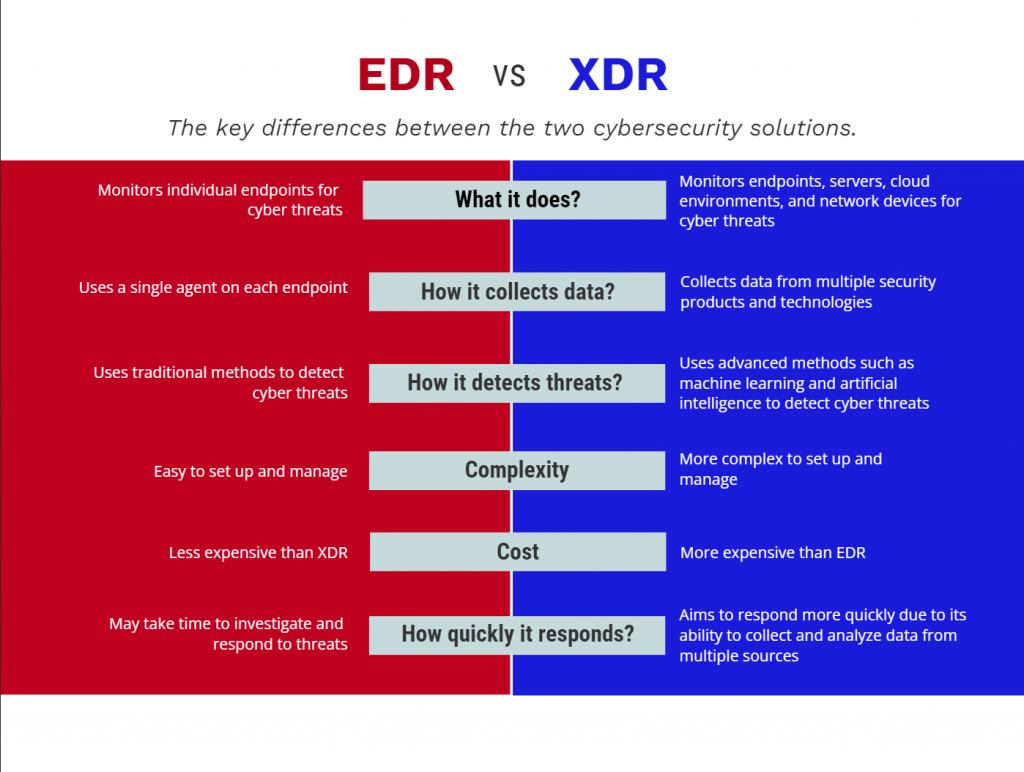
\includegraphics[width=0.9\textwidth]{img/edr-xdr-comparison.png}
    \caption{EDR ve XDR Platformları Arasındaki Temel Farklar ve Yetenekler}
    \label{fig:edr-xdr-comparison}
\end{figure}

\begin{longtable}{|p{4cm}|p{4cm}|p{4cm}|p{4cm}|}
\hline
\textbf{Kriterler} & \textbf{Endpoint Protection Platform (EPP)} & \textbf{Endpoint Detection and Response (EDR)} & \textbf{Extended Detection and Response (XDR)} \\
\hline
\textbf{Kapsam} & Yalnızca uç nokta cihazları (PC, sunucu). & Yalnızca uç nokta cihazları (PC, sunucu). & Uç nokta, ağ, e-posta, bulut, kimlik. \\
\hline
\textbf{Temel Yetenek} & Önleme odaklı koruma & Tespit ve yanıt & Çoklu katman tespit \\
\hline
\textbf{Hedef} & Tehdit engelleme & Gelişmiş tehdit tespiti & Bütünsel görünürlük \\
\hline
\textbf{Mimari} & Bulut tabanlı veya şirket içi. & Bulut tabanlı veya şirket içi. & Genellikle bulut tabanlı bir hizmet (SaaS). \\
\hline
\textbf{Yanıt} & Otomatik engelleme & Manuel iyileştirme & Orkestrasyonlu yanıt \\
\hline
\textbf{Notlar} & İlk savunma hattı & Tehdit avcılığı & Kapsamlı entegrasyon \\
\hline
\end{longtable}

\section{İşletim Sistemi Güvenliği ve Sertleştirme (Hardening)}

Bir sistemin sertleştirilmesi (hardening), saldırı yüzeyini en aza indirmek ve güvenlik açıklarını gidermek için sistemin konfigürasyonunu ve ayarlarını güçlendirme sürecidir. Bu süreç, sadece güvenlik yazılımları kurmakla sınırlı kalmamakta, aynı zamanda işletim sistemi seviyesindeki tüm varsayılan ve potansiyel zafiyetlerin giderilmesini içermektedir. CIS Benchmarks gibi endüstri standartları, bu süreç için yol gösterici rol oynamaktadır.

Windows işletim sistemini güvenli hale getirmek, hem yerleşik güvenlik özelliklerini doğru bir şekilde yapılandırmayı hem de sürekli güncellemelerle bilinen zafiyetleri gidermeyi gerektirmektedir. Bir Windows sisteminin sertleştirilmesi için aşağıdaki temel adımlar izlenebilmektedir:
\begin{itemize}
    \item \textbf{Parola Politikaları:} Güçlü parola politikaları, bir sistemin temel güvenlik duruşu için hayati öneme sahiptir. Bu politikalar, parolaların minimum uzunluğunu, karmaşıklık gereksinimlerini, maksimum ve minimum geçerlilik sürelerini ve hesap kilitleme eşiğini belirlemektedir.
    \item \textbf{Kullanıcı Hesap Yönetimi:} Varsayılan yönetici ve misafir hesaplarının yeniden adlandırılması veya devre dışı bırakılması, saldırganların otomatik araçlarla bu hesapları hedef almasını zorlaştırmaktadır.
    \item \textbf{Uzak Erişimin Kısıtlanması:} RDP gibi uzak erişim servisleri, yalnızca gerektiğinde ve güvenli kanallardan (VPN veya jump server) erişime açık olmalıdır.
    \item \textbf{Yerleşik Güvenlik Özellikleri:} Windows Defender Antivirus, SmartScreen ve Exploit Protection gibi yerleşik özelliklerin etkinleştirilmesi, kötü amaçlı yazılımlara ve web tabanlı tehditlere karşı temel koruma sağlamaktadır.
    \item \textbf{PowerShell Sertleştirmesi:} PowerShell, Windows ortamında sıklıkla kötü amaçlı komut dosyalarının çalıştırılması için kullanılmaktadır. PowerShell'in kendisini güvence altına almak için çalıştırma politikaları (Execution Policy) uygulanmakta ve komut betiği loglaması (Script Block Logging) etkinleştirilmektedir.
\end{itemize}

\subsection{Pratik PowerShell Sertleştirme Script Örnekleri}

Windows sistemleri için güvenlik ayarlarını otomatikleştirmek üzere PowerShell scriptleri kullanılabilmektedir. Aşağıda, temel bir sertleştirme senaryosu için örnekler sunulmuştur.

\begin{enumerate}
    \item \textbf{Parola Politikalarını Yapılandırma:}
    \begin{verbatim}
# Parola geçmişini 24 olarak ayarla
secedit /configure /cfg C:\temp\policy.inf \
       /db C:\temp\policy.sdb /areas SECURITYPOLICY
# Parola geçmişi 24
Set-ItemProperty -Path "HKLM:\SOFTWARE\Microsoft\...\PasswordPolicy" `
    -Name "PasswordHistory" -Value 24

# Minimum parola yaşı 1 gün
Set-ItemProperty -Path "HKLM:\SOFTWARE\Microsoft\...\PasswordPolicy" `
    -Name "MinimumPasswordAge" -Value 1

# Maksimum parola yaşı 60 gün  
Set-ItemProperty -Path "HKLM:\SOFTWARE\Microsoft\...\PasswordPolicy" `
    -Name "MaximumPasswordAge" -Value 60
    \end{verbatim}
    \item \textbf{PowerShell Çalıştırma Politikasını Ayarlama:}
    \texttt{Set-ExecutionPolicy} komutu, PowerShell'in scriptleri çalıştırmasına izin veren koşulları kontrol etmektedir. \texttt{RemoteSigned} politikası, yerel olarak oluşturulan scriptlerin çalışmasına izin verirken, internetten indirilenlerin güvenilir bir yayıncı tarafından imzalanmasını zorunlu kılmaktadır.
    \texttt{Set-ExecutionPolicy -ExecutionPolicy RemoteSigned -Scope LocalMachine}
    \item \textbf{PowerShell Loglamasını Etkinleştirme:}
    Script bloklarının ve modül faaliyetlerinin Windows olay günlüğüne kaydedilmesini sağlamak, adli inceleme ve tehdit avcılığı için kritik bir adımdır. Bu ayar GPO üzerinden kolayca yapılandırılabilmektedir.
\end{enumerate}

\subsection{Linux Güvenliği: SELinux ve AppArmor}

Linux işletim sistemleri, geleneksel isteğe bağlı erişim kontrolü (DAC) modelinin ötesine geçen, zorunlu erişim kontrolü (MAC) mekanizmalarıyla güçlendirilmektedir. Bu mekanizmalar, kötü amaçlı yazılımların ve yetkisiz kullanıcıların sisteme zarar vermesini engellemektedir. Bu alandaki en yaygın iki teknoloji \textbf{SELinux} ve \textbf{AppArmor}'dur.

\begin{itemize}
    \item \textbf{SELinux (Security-Enhanced Linux):} ABD Ulusal Güvenlik Ajansı (NSA) tarafından geliştirilen SELinux, "label-based" (etiket tabanlı) bir model kullanmaktadır. Her dosya, süreç ve kullanıcı, güvenlik bağlamı (security context) adı verilen bir etiketle etiketlenmektedir. SELinux politikaları, bu etiketler arasındaki etkileşimleri sıkı bir şekilde tanımlamaktadır. Bu model, son derece granüler ve katı bir kontrol sağladığı için kurumsal ve yüksek güvenlik gereksinimleri olan ortamlar için idealdir. Ancak, öğrenme eğrisi daha diktir ve politika yönetimi karmaşık olabilmektedir.
    \item \textbf{AppArmor (Application Armor):} "Path-based" (yol tabanlı) bir model kullanan AppArmor, uygulamalara, dosya yollarına dayalı profiller atamaktadır. Bu profiller, bir uygulamanın hangi dosyalara ve kaynaklara erişebileceğini net bir şekilde belirlemektedir. AppArmor, SELinux'a göre daha kolay yönetilebilir ve daha basit bir öğrenme eğrisine sahiptir, bu da onu masaüstü sistemler ve daha basit sunucu ortamları için iyi bir seçenek haline getirmektedir.
\end{itemize}

\textbf{Konteyner Güvenliği:} Docker ve Kubernetes gibi konteyner teknolojileri, uygulamaları izole etse de, aynı işletim sistemi çekirdeğini paylaşmaktadırlar. Bu durum, bir güvenlik açığının tüm konteynerli sistemi etkileme potansiyelini taşımaktadır. 

SELinux ve AppArmor, konteyner güvenliğini artırmak için kullanılmaktadır. Örneğin, Kubernetes, konteynerlerin AppArmor profilleriyle çalışmasını sağlayarak ek bir izolasyon katmanı ekleyebilmektedir.

\subsection{Pratik Komut Örnekleri}

\begin{itemize}
    \item \textbf{SELinux Modunu Kontrol Etme:} \texttt{getenforce} komutu, \\
    SELinux'un mevcut modunu (\texttt{Enforcing}, \texttt{Permissive} \\
    veya \texttt{Disabled}) göstermektedir. \texttt{sestatus} komutu, \\
    daha detaylı bir durum raporu sunmaktadır.
    \item \textbf{SELinux Modunu Değiştirme:} Modu geçici olarak \texttt{Permissive} (yalnızca loglama, engelleme yok) moda geçirmek için: \texttt{sudo setenforce 0} Modu tekrar \texttt{Enforcing} moda getirmek için: \texttt{sudo setenforce 1}. Kalıcı değişiklikler için \texttt{/etc/selinux/config} dosyası düzenlenmektedir.
    \item \textbf{AppArmor Durumunu Kontrol Etme:} \texttt{sudo aa-status} komutu, etkin ve şikayet modundaki profilleri listelemektedir.
\end{itemize}

\subsection{SELinux vs. AppArmor Karşılaştırması}

\begin{longtable}{|p{4.5cm}|p{4.5cm}|p{4.5cm}|}

\hline

\textbf{Kriterler} & \textbf{SELinux (Security-Enhanced Linux)} & \textbf{AppArmor (Application Armor)} \\
\hline
\textbf{Güvenlik Modeli} & Etiket tabanlı (Label-based). Her varlığa güvenlik etiketi atar. & Yol tabanlı (Path-based). Kuralları dosya yollarına atar. \\
\hline
\textbf{Öğrenme Eğrisi} & Oldukça dik ve karmaşıktır. Detaylı politika yönetimi gerektirir. & Genellikle daha kolay ve basittir. Profiller daha anlaşılırdır. \\
\hline
\textbf{Kontrol Seviyesi} & Çok granüler ve katıdır. Kullanıcılar, süreçler ve objeler üzerinde detaylı kurallar tanımlar. & Uygulama bazlı daha statik kontrol sağlar. Önceden tanımlanmış davranışlar için daha uygundur. \\
\hline
\textbf{Esneklik} & Dinamik ortamlar için daha esnektir. & Dinamik ortamlarda daha az idealdir. \\
\hline
\textbf{Varsayılan Dağıtım} & Fedora, CentOS/RHEL gibi dağıtımlarda varsayılan olarak gelir. & Ubuntu, SUSE gibi dağıtımlarda varsayılan olarak gelir. \\
\hline
\textbf{İdeal Kullanım} & Yüksek güvenlikli ve karmaşık kurumsal ortamlar, konteyner platformları. & Masaüstü sistemleri ve yönetim kolaylığının öncelikli olduğu sunucular. \\
\hline
\end{longtable}

\subsection{macOS Security Architecture ve Enterprise Management}

macOS, donanım ve yazılım katmanına entegre edilmiş sağlam bir güvenlik mimarisi sunmaktadır. Bu mimari, kullanıcı verilerini korumaya ve kötü amaçlı yazılımlara karşı sistemi sertleştirmeye odaklanmaktadır. Apple'ın kendi tasarladığı M serisi çipler, bu güvenlik altyapısının temelini oluşturmaktadır.

\textbf{Temel Güvenlik Özellikleri:}
\begin{itemize}
    \item \textbf{Secure Enclave:} Ana işlemciden fiziksel olarak izole edilmiş, hassas kullanıcı verilerini (parola ve biyometrik veriler) koruyan özel bir yardımcı işlemcidir. Bu yonga, ana işlemci saldırıya uğrasa bile hassas verilerin güvenliğini sağlamaktadır.
    \item \textbf{System Integrity Protection (SIP):} SIP, yönetici yetkilerine sahip süreçlerin bile kritik sistem dosyalarını ve klasörlerini değiştirmesini engellemektedir. Bu, çekirdek ve sistem dosyalarına yönelik saldırıları önlemektedir.
    \item \textbf{Gatekeeper:} İnternetten indirilen uygulamaların, bilinen kötü amaçlı yazılımlara karşı Apple tarafından imzalanmış ve onaylanmış olup olmadığını denetlemektedir. Bu, kullanıcıları güvenilmeyen yazılımlara karşı korumaktadır.
    \item \textbf{FileVault 2:} Diskin tamamını şifreleyerek cihaz çalınsa veya kaybolsa bile verilerin güvenliğini sağlamaktadır. Apple Silicon çipler, bu şifreleme işlemini donanım seviyesinde destekleyerek daha da ileri bir güvenlik katmanı sunmaktadır.
\end{itemize}

\textbf{Kurumsal Yönetim:}

macOS cihazlarının kurumsal ortamda yönetimi, Mobil Cihaz Yönetimi (MDM) çözümleri aracılığıyla gerçekleştirilmektedir. MDM, yöneticilere merkezi bir platformdan cihazlara güvenlik politikaları uygulamalarına, uygulama dağıtmalarına ve envanter yönetimi yapmalarına olanak tanımaktadır. Bu araçlar, macOS'in yerleşik güvenlik özelliklerini tamamlayarak cihazların kuruluş politikalarına uygunluğunu sağlamaktadır.

\subsection{Mobil İşletim Sistemleri: iOS/Android Güvenlik Modelleri}

Mobil cihazlar, kurumsal kaynaklara erişimin ana kapısı haline geldiğinden, mobil işletim sistemlerinin güvenlik modelleri hayati önem taşımaktadır. iOS ve Android, farklı yaklaşımlarla güvenliği sağlamaktadır.

\begin{itemize}
    \item \textbf{iOS Güvenlik Modeli:}
    \begin{itemize}
        \item \textbf{Kapalı Ekosistem (Walled Garden):} iOS, uygulamaların yalnızca Apple'ın App Store'u üzerinden dağıtılmasına izin vermektedir. Her uygulama, yayınlanmadan önce katı bir inceleme sürecinden geçmektedir. Bu yaklaşım, zararlı uygulamaların kullanıcılara ulaşmasını zorlaştırmaktadır.
        \item \textbf{Sandbox (Korumalı Alan):} Her uygulama, diğer uygulamalardan ve sistemden izole edilmiş kendi "sandbox" ortamında çalışmaktadır. Bu, bir uygulamanın güvenliğinin aşılması durumunda diğer uygulamalara ve hassas verilere zarar vermesini engellemektedir.
        \item \textbf{İzin Modeli:} Uygulamalar, kameraya, mikrofona veya konumlara erişim gibi hassas verilere erişim için kullanıcıdan açık izin istemektedir.
    \end{itemize}
    \item \textbf{Android Güvenlik Modeli:}
    \begin{itemize}
        \item \textbf{Açık Ekosistem:} Android, uygulamaların Google Play Store'un yanı sıra üçüncü parti mağazalardan da yüklenebilmesine olanak tanımaktadır. Bu esneklik, geliştiriciler için daha fazla özgürlük sağlarken, kullanıcılar için potansiyel riskleri de artırmaktadır.
        \item \textbf{Güvenlik Katmanları:} Android, sandbox modelini kullanmakta ve her uygulamayı kendi kullanıcı kimliğiyle çalıştırmaktadır. Ayrıca, Google Play Protect gibi hizmetler, kötü amaçlı yazılımlara karşı ek bir koruma sağlamaktadır.
        \item \textbf{BYOD Politikaları:} Android for Work ve Samsung Knox gibi platformlar, kurumsal uygulamaları ve verileri kişisel verilerden ayırmak için iş profilleri oluşturma yeteneği sunmaktadır.
    \end{itemize}
\end{itemize}

\subsection{Sanallaştırma Güvenliği: Hypervisor ve VM İzolasyonu}

Sanallaştırma, bir fiziksel sunucu üzerinde birden fazla sanal makinenin (VM) çalıştırılmasına olanak tanıyarak kaynak kullanımını optimize etmektedir. Bu mimarinin güvenliği, VM'ler arasında izolasyonu sağlayan ve fiziksel donanıma erişimi kontrol eden temel bileşen olan \textbf{Hypervisor}'a bağlıdır.

\textbf{Hypervisor Türleri ve Güvenlik:}
\begin{itemize}
    \item \textbf{Tip 1 (Bare-metal) Hypervisor:} Fiziksel donanım üzerinde doğrudan çalışmaktadır (örneğin, VMware ESXi, Microsoft Hyper-V). Bu tür hypervisor'lar, bir aracı işletim sistemi katmanına ihtiyaç duymadığı için yüksek düzeyde güvenlik ve performans sağlamaktadır.
    \item \textbf{Tip 2 (Hosted) Hypervisor:} Bir ana işletim sistemi üzerinde bir uygulama olarak çalışmaktadır (örneğin, VMware Workstation, VirtualBox). Kurulumu daha kolay olmasına rağmen, güvenliği ana işletim sisteminin güvenliğine bağlıdır, bu da onu saldırılara karşı daha hassas hale getirebilmektedir.
\end{itemize}

\textbf{VM İzolasyon Teknikleri:}
\begin{itemize}
    \item \textbf{Donanım Soyutlama:} Hypervisor, her VM'ye sanal CPU, bellek ve depolama gibi sanal donanım kaynakları sağlamaktadır. Bu soyutlama, VM'lerin birbirlerinin kaynaklarına doğrudan erişimini engellemektedir.
    \item \textbf{Bellek ve Ağ Segmentasyonu:} Her VM'ye kendi bellek segmenti ve sanal ağ arayüzü tahsis edilmektedir. Bu segmentasyon, bir VM'nin belleğindeki verilere veya ağ trafiğine diğer VM'lerin erişmesini önlemektedir, bu da yanal hareket gibi saldırı türlerini zorlaştırmaktadır.
    \item \textbf{CPU Planlama:} Hypervisor, her VM için CPU zamanını planlayarak hiçbir VM'nin CPU kaynaklarını tekeline almasını engellemektedir.
\end{itemize}

\textbf{Hyper-V Sertleştirme Adımları}

Bir Hyper-V ortamının güvenliğini sağlamak için aşağıdaki adımlar izlenmelidir:

\begin{enumerate}
    \item \textbf{Ana Bilgisayarı (Host) Minimal Tutma:} Hyper-V ana bilgisayarı, yalnızca sanallaştırma için kullanılmalı ve dosya sunucusu veya etki alanı denetleyicisi gibi ek roller yüklenmemelidir.
    \item \textbf{Güvenlik Duvarı Konfigürasyonu:} Yalnızca gerekli portlar açılmalı ve yönetim portlarına (örneğin, RDP) yalnızca kısıtlı ağlardan (VPN gibi) erişime izin verilmelidir.
    \item \textbf{Anti-malware Kurulumu:} Hyper-V ana bilgisayarında anti-malware yazılımı çalıştırılmalı ve VM dosyaları (VHD/VHDX) tarama istisnalarına eklenmelidir.
    \item \textbf{En Az Yetki İlkesi:} Hyper-V yönetimine erişim, yalnızca gerekli kullanıcılarla sınırlandırılmalıdır.
    \item \textbf{VM Güvenliği:} Yeni oluşturulan VM'ler, üretime geçmeden önce tıpkı fiziksel bir sunucu gibi sertleştirilmelidir. Güvenli Önyükleme (Secure Boot) etkinleştirilmeli ve güncel yamalar uygulanmalıdır.
\end{enumerate}

\section{Sistem Konfigürasyon Yönetimi ve Uyum}

Sistem konfigürasyon yönetimi, bir kuruluşun ağındaki tüm sistemlerin ve cihazların yapılandırmalarını standartlaştırma, izleme ve yönetme sürecidir. Bu, güvenlik politikalarının tutarlı bir şekilde uygulanmasını sağlar, yanlış yapılandırmalardan kaynaklanan güvenlik açıklarını azaltır ve operasyonel verimliliği artırır. Uyum (compliance) ise, bir kuruluşun belirli endüstri standartlarına, yasal düzenlemelere ve en iyi uygulamalara uygunluğunu sağlama sürecidir.

\subsection{Güvenlik Temel Konfigürasyon Standartları (CIS Benchmarks)}

\begin{figure}[H]
    \centering
    
\includegraphics[width=0.5\textwidth]{img/logo_cis.png}
    \caption{Center for Internet Security (CIS) Logosu}
    \label{fig:cis-logo}
\end{figure}

CIS Benchmarks, Center for Internet Security (CIS) tarafından geliştirilen ve işletim sistemleri, uygulamalar, ağ cihazları ve bulut altyapıları için konsensüs tabanlı güvenlik konfigürasyon önerileridir. Bu standartlar, bir organizasyonun güvenlik duruşunu geliştirmesine, zafiyetleri azaltmasına ve yasal düzenlemelerle (GDPR, HIPAA gibi) uyumunu sağlamasına yardımcı olmaktadır.

\textbf{Level 1 vs. Level 2}

CIS Benchmarks, organizasyonların ihtiyaçlarına göre farklı seviyelerde uygulanabilmektedir.

\begin{itemize}
    \item \textbf{Level 1 (Temel):} Hizmet ve işlevsellik üzerinde minimal etkiye sahip temel güvenlik gereksinimlerini içermektedir. Sınırlı siber güvenlik kaynaklarına sahip küçük ve orta ölçekli işletmeler için uygundur.
    \item \textbf{Level 2 (Kapsamlı):} Daha kapsamlı ve sıkı güvenlik gereksinimleri sunmaktadır. Uygulaması daha fazla test ve operasyonel değişiklik gerektirebilmektedir. Hassas verileri işleyen, kritik altyapıya sahip veya yüksek siber risk altındaki organizasyonlar (finans, sağlık, kamu) için tasarlanmıştır.
\end{itemize}

Bir organizasyonun hangi seviyeyi uygulayacağına karar verirken, kendi risk profilini, iş gereksinimlerini ve yasal uyumluluk zorunluluklarını dikkate alması gerekmektedir.

\subsection{Grup İlkesi Yönetimi ve Güvenlik Şablonları}

Grup İlkesi Yönetimi (GPO), Microsoft Active Directory (AD) ortamında, Windows makineleri için merkezi konfigürasyon ve güvenlik politikalarının uygulanmasını sağlayan güçlü bir araçtır. GPO'lar, yöneticilerin tüm alan (domain) veya belirli organizasyonel birim (OU) içindeki bilgisayarlara ve kullanıcılara tek bir merkezden ayarlar uygulamasına olanak tanımaktadır.

\textbf{Temel Uygulama Alanları:}
\begin{itemize}
    \item \textbf{Parola Politikaları:} GPO, parola karmaşıklığı, uzunluğu ve geçerlilik süresi gibi ayarları tüm kullanıcılar için zorunlu kılmaktadır.
    \item \textbf{Erişim Kısıtlamaları:} Yönetim paneli, komut satırı veya belirli uygulamalara erişimi kısıtlamak için kullanılabilmektedir.
    \item \textbf{Güvenlik Şablonları:} Önceden yapılandırılmış güvenlik ayarları setlerini içeren şablonlar, tutarlı ve standartlaştırılmış güvenlik politikalarının uygulanmasını kolaylaştırmaktadır. Örneğin, bir güvenlik şablonu, bir Windows sistemini CIS Benchmarks'e göre sertleştirmek için tüm gerekli ayarları içerebilmektedir.
\end{itemize}

\subsection{Konfigürasyon Yönetim Araçları (Ansible, Puppet, Chef)}

Konfigürasyon yönetim araçları, altyapıyı "kod olarak" (Infrastructure as Code - IaC) yöneterek, güvenlik politikalarının ve konfigürasyonların otomatik, tekrarlanabilir ve tutarlı bir şekilde uygulanmasını sağlamaktadır. Bu otomasyon, güvenlik ekiplerinin iş yükünü azaltmakta ve manuel hataların neden olduğu güvenlik açıklarını gidermektedir.

\begin{itemize}
    \item \textbf{Ansible:} \textbf{Ajansız (agentless)} bir mimariye sahiptir, yani yönetilen makinelerde bir ajan yazılımı gerektirmez. Python ve YAML tabanlı "playbook" adı verilen dosyaları kullanarak SSH veya WinRM üzerinden uzaktan komutları çalıştırmaktadır. Kurulumu kolaydır ve küçük ile orta ölçekli ortamlar için idealdir.
    \item \textbf{Puppet:} \textbf{Ajan tabanlı (agent-based)} bir mimariye sahiptir. Yönetilen her makinede bir ajan (Puppet Agent) çalışmaktadır ve bu ajan, merkezi bir sunucudan (Puppet Master) konfigürasyonları düzenli aralıklarla çekmektedir.
    \item \textbf{Chef:} Puppet gibi \textbf{ajan tabanlı} bir mimari kullanmaktadır. Konfigürasyonlar, Ruby diliyle yazılmış "cookbook" ve "recipe" adı verilen dosyalarda tanımlanmaktadır.
\end{itemize}

\subsection{Konfigürasyon Yönetim Araçları Karşılaştırması}

\begin{longtable}{|p{4cm}|p{4cm}|p{4cm}|p{4cm}|}
\hline
\textbf{Kriterler} & \textbf{Ansible} & \textbf{Puppet} & \textbf{Chef} \\
\hline
\textbf{Mimari} & Ajansız (Agentless). & Ajan tabanlı (Agent-based). & Ajan tabanlı (Agent-based). \\
\hline
\textbf{İletişim Modeli} & İtme (Push) modeli. Komutları hedef makinelerde çalıştırır. & Çekme (Pull) modeli. Ajanlar sunucudan konfigürasyonları çeker. & Çekme (Pull) modeli. Ajanlar sunucudan konfigürasyonları çeker. \\
\hline
\textbf{Dil} & YAML tabanlı "Playbook"lar. & Puppet DSL. & Ruby tabanlı "Cookbook"lar. \\
\hline
\textbf{Öğrenme Zorluğu} & Diğerlerine göre daha kolaydır. & Öğrenme eğrisi daha diktir. & Ruby bilgisi gerektirdiğinden zor olabilir. \\
\hline
\textbf{İdeal Kullanım} & Hızlı dağıtımlar, küçük ortamlar ve ağ cihazı yönetimi. & Karmaşık, büyük kurumsal ortamlar için tutarlılık ve otomasyon. & Özelleştirme ve esneklik gerektiren DevOps ortamları. \\
\hline
\end{longtable}

\subsection{Sürekli Uyum İzleme ve Drift Tespiti}

Bir sistemin konfigürasyonu, manuel değişiklikler, yamalar veya diğer faktörler nedeniyle zamanla başlangıçtaki güvenli durumundan sapabilmektedir. Bu duruma \textbf{konfigürasyon kayması (drift)} denilmektedir ve güvenlik açıkları, istikrarsızlık ve uyumluluk ihlallerine yol açabilmektedir.

\textbf{Drift Tespiti:}

Drift tespiti, bir sistemin gerçek durumunu, kodda (IaC) tanımlanan "istenilen durumla" sürekli olarak karşılaştıran bir mekanizmadır. Bu, manuel değişikliklerin sistemin güvenliğinden sapıp sapmadığını belirlemeyi sağlamaktadır. GitOps gibi metodolojiler, tüm altyapı konfigürasyonlarını Git versiyon kontrol sisteminde saklayarak ve canlı ortamı bu kodla sürekli senkronize ederek drift'i önlemektedir.

\textbf{Araçlar ve Teknikler:}
\begin{itemize}
    \item \textbf{IaC Araçları:} Terraform, OpenTofu veya AWS CloudFormation gibi altyapı kodu araçları, \texttt{terraform plan} gibi komutlarla canlı ortamdaki değişiklikleri tespit edebilmektedir.
    \item \textbf{Konfigürasyon Yönetimi:} Puppet ve Chef InSpec gibi araçlar, düzenli taramalarla sistemlerin belirlenen güvenlik politikalarına (örneğin, CIS Benchmarks) uygunluğunu sürekli denetleyebilmektedir.
    \item \textbf{Otomatik İyileştirme:} Drift tespit edildiğinde, ArgoCD veya Chef Automate gibi çözümler, sistemi otomatik olarak istenilen duruma geri döndürerek (remediation) tutarlılığı sağlamaktadır.
\end{itemize}

\subsection{Yama Yönetimi Otomasyonu ve Test Prosedürleri}

Yama yönetimi (patch management), işletim sistemlerinde ve uygulamalarda bulunan güvenlik açıklarını düzeltmek için güncellemeleri yönetme sürecidir. Bu süreç, siber güvenlik stratejisinin temel bir bileşenidir çünkü bilinen zafiyetler, saldırganlar için en yaygın giriş noktalarından birini oluşturmaktadır.

Yama yönetimi süreci aşağıdaki adımları içermektedir:

\begin{enumerate}
    \item \textbf{Varlık Yönetimi:} Güncelleme gerektiren tüm donanım ve yazılımların envanteri çıkarılmalıdır.
    \item \textbf{Zafiyet Değerlendirmesi:} Düzenli zafiyet taramalarıyla, sistemlerdeki mevcut güvenlik açıkları tespit edilmelidir.
    \item \textbf{Yama İzleme:} Yazılım üreticilerinden gelen yeni yamalar ve güvenlik bültenleri sürekli olarak takip edilmelidir.
    \item \textbf{Test Etme:} En kritik adım, yamaları üretim ortamına uygulamadan önce bir test ortamında denemektir. Bu ortam, canlı sistemlerin konfigürasyonunu ve kullanılan üçüncü parti uygulamaları taklit etmelidir. Test, yamanın beklenmedik yan etkilere veya uygulama kesintilerine neden olup olmadığını belirlemek için yapılmaktadır.
    \item \textbf{Otomasyon:} Yama yönetimini otomatikleştiren çözümler, süreci hızlandırmakta ve manuel müdahale ihtiyacını azaltmaktadır. Otomatik dağıtım araçları, yamaların doğru zamanda ve doğru sistemlere uygulanmasını sağlamaktadır.
    \item \textbf{Doğrulama:} Yama uygulandıktan sonra, zafiyetin gerçekten giderildiğinden emin olmak için ek taramalar yapılmalıdır.
\end{enumerate}

\section{Mobile Device Management (MDM) ve BYOD Güvenliği}

Mobil Cihaz Yönetimi (MDM), bir kuruluşun çalışanlarına ait veya şirket tarafından sağlanan mobil cihazları (akıllı telefonlar, tabletler) merkezi olarak yönetmesini, güvenliğini sağlamasını ve izlemesini sağlayan bir yazılım çözümüdür. Kendi Cihazını Getir (BYOD) politikaları, çalışanların kişisel cihazlarını iş amaçlı kullanmalarına izin verir. Bu, esneklik ve maliyet tasarrufu sağlarken, aynı zamanda önemli güvenlik riskleri de yaratır.

MDM çözümleri, cihaz kaydı, uzaktan silme, şifre politikaları, uygulama yönetimi ve güvenlik güncellemeleri gibi özellikler sunarak, mobil cihazların güvenli bir şekilde yönetilmesini sağlamaktadır. Ayrıca, BYOD politikalarıyla birlikte kullanıldığında, çalışanların kişisel verilerini korurken kurumsal verilerin güvenliğini de garanti altına almaktadır.

\subsection{Enterprise Mobility Management (EMM) Çözümleri}

Kurumsal Mobilite Yönetimi (EMM), organizasyonun mobil cihazlarını, uygulamalarını ve verilerini yönetmek ve güvence altına almak için kullanılan kapsamlı bir çerçevedir. EMM, aşağıdaki bileşenleri bir araya getirmektedir:

\begin{itemize}
    \item \textbf{Mobil Cihaz Yönetimi (MDM):} Cihazın tamamını (envanter, konfigürasyon, güvenlik politikaları) yönetmeye odaklanır.
    \item \textbf{Mobil Uygulama Yönetimi (MAM):} Yalnızca kurumsal uygulamaları ve verileri yönetmeye odaklanır.
    \item \textbf{Mobil İçerik Yönetimi (MCM):} Kurumsal verilere güvenli bir şekilde erişim ve paylaşım sağlar.
\end{itemize}

EMM, organizasyonlara mobil varlıklarını tek bir platformdan yönetme, hassas verileri gelişmiş şifreleme ve veri kaybı önleme (DLP) önlemleriyle koruma yeteneği sunmaktadır.

\subsection{Mobil Uygulama Yönetimi (MAM) Stratejileri}

MAM, özellikle BYOD ortamlarında çalışan gizliliğini korumak için tasarlanmış bir yaklaşımdır. Cihazın tamamını kontrol etmeden, sadece kurumsal uygulamaları ve bu uygulamalardaki verileri korumaya odaklanmaktadır.

\textbf{Temel MAM Özellikleri:}
\begin{itemize}
    \item \textbf{Uygulama Koruma Politikaları:} Hassas kurumsal verilerin \\
    kişisel uygulamalara (örneğin, OneDrive'dan WhatsApp'a) \\
    kopyalanmasını veya yapıştırılmasını engellemektedir.
    \item \textbf{Seçici Veri Silme:} Cihaz çalındığında veya bir çalışan işten ayrıldığında, cihazdaki kişisel verileri silmeden yalnızca kurumsal verilerin ve uygulamaların uzaktan silinmesini sağlamaktadır.
    \item \textbf{Erişim Kontrolü:} Kurumsal uygulamalara erişim için bir PIN veya biyometrik doğrulama gereksinimi gibi politikalar uygulanabilmektedir.
\end{itemize}

Bu stratejiler, çalışanların kişisel cihazlarında kurumsal verilerle güvenli bir şekilde çalışmasına olanak tanımaktadır.

\subsection{MDM vs. MAM Karşılaştırması}

\begin{longtable}{|p{4.5cm}|p{4.5cm}|p{4.5cm}|}
\hline
\textbf{Kriterler} & \textbf{Mobile Device Management (MDM)} & \textbf{Mobile Application Management (MAM)} \\
\hline
\textbf{Kontrol Seviyesi} & Cihazın tamamını yönetir. & Yalnızca belirli uygulamaları ve verilerini yönetir. \\
\hline
\textbf{Yönetim Odağı} & Cihazın kendisi, konfigürasyonu, ağ ayarları, güvenlik politikaları. & Uygulamalar, uygulama verileri ve veri hareket kuralları. \\
\hline
\textbf{Kullanım Alanı} & Şirkete ait cihazlar (Corporate-owned devices). & Çalışana ait cihazlar (BYOD) ve özel uygulamalar. \\
\hline
\textbf{BYOD Uyumluluğu} & Genellikle kullanıcı gizliliği endişesi nedeniyle sınırlı. & Kullanıcının kişisel verilerini koruduğu için BYOD dostudur. \\
\hline
\textbf{Veri Silme} & Tüm cihazı fabrika ayarlarına döndüren tam silme. & Yalnızca kurumsal verileri silen seçici silme. \\
\hline
\end{longtable}

\subsection{Konteynerleştirme ve İş Profili Yönetimi}

BYOD güvenliği için kritik bir strateji de konteynerleştirme teknolojisidir. Konteynerleştirme, bir cihazda kişisel verileri ve kurumsal verileri birbirinden izole edilmiş sanal alanlarda ayırmaktadır.

\textbf{İş Profili Yönetimi:}

Android Enterprise gibi platformlar, cihaz üzerinde bir "iş profili" oluşturmaktadır. Bu profil, kişisel uygulamalardan ve verilerden tamamen izole edilmiştir. Tüm kurumsal uygulamalar ve veriler bu profilin içinde yer alır ve kuruluş tarafından yönetilmektedir. Bu yaklaşım, bir yandan çalışan mahremiyetini korurken, diğer yandan hassas kurumsal verilerin güvenliğini garanti altına almaktadır. Bu izolasyon, veri sızıntısını ve zararlı yazılımların kurumsal alana bulaşmasını engellemektedir.

\subsection{Mobil Tehdit Savunması (MTD) Entegrasyonu}

Mobil Tehdit Savunması (MTD), mobil cihazlara yönelik oltalama (phishing) saldırıları, kötü amaçlı yazılımlar ve sıfır-gün tehditleri gibi dinamik siber tehditlere karşı gerçek zamanlı koruma sağlayan bir güvenlik stratejisidir. MTD çözümleri, mobil cihazların, ağ bağlantılarının ve yüklü uygulamaların güvenlik seviyesini sürekli olarak analiz etmektedir.

MTD'nin en önemli özelliklerinden biri, MDM çözümleriyle olan entegrasyonudur. MTD, bir cihazın jailbreak yapıldığını veya şüpheli bir ağa bağlı olduğunu tespit ettiğinde, MDM'ye bu durumu bildirmektedir. MDM, bu bilgilere dayanarak cihazın kurumsal kaynaklara erişimini engelleyebilmekte veya önceden tanımlanmış diğer yanıt eylemlerini tetikleyebilmektedir. Bu entegrasyon, mobil cihazlar için hem yönetim (MDM) hem de savunma (MTD) yeteneklerini birleştiren katmanlı bir güvenlik modeli oluşturmaktadır.

\subsection{Uzaktan Silme (Remote Wipe) ve Veri Sızıntısı Önleme}

Uzaktan silme, bir mobil cihaz çalındığında, kaybolduğunda veya bir çalışanın işten ayrılması durumunda, cihazdaki hassas verilerin uzaktan silinmesini sağlayan kritik bir güvenlik özelliğidir. Bu özellik, veri sızıntısını (DLP - Data Leakage Prevention) önlemek için son savunma hattını temsil etmektedir.

\textbf{Kullanım Senaryoları:}
\begin{itemize}
    \item \textbf{Cihaz Hırsızlığı veya Kaybı:} Bir cihazın yanlış ellere düşmesi durumunda, kurumsal verilerin yetkisiz erişime karşı korunmasını sağlamaktadır.
    \item \textbf{Çalışan Ayrılışı:} Şirketten ayrılan bir çalışanın cihazında kalan kurumsal verilerin silinmesi için kullanılmaktadır.
    \item \textbf{İç Tehditler:} Kötü niyetli bir çalışanın şirkete ait verileri ele geçirmesi durumunda, verilerin uzaktan silinmesini sağlamaktadır.
\end{itemize}

\textbf{Seçici (Selective) vs. Tam (Full) Silme:}
\begin{itemize}
    \item \textbf{Tam Silme (Full Wipe):} Cihazdaki tüm veriyi kalıcı olarak silerek cihazı fabrika ayarlarına döndürmektedir.
    \item \textbf{Seçici Silme (Selective Wipe):} BYOD ortamları için idealdir. Yalnızca kurumsal verileri ve uygulamaları silmekte, kullanıcının kişisel fotoğraflarını, mesajlarını veya diğer verilerini korumaktadır.
\end{itemize}

Uzaktan silme eylemleri, MDM çözümleri aracılığıyla tek bir yönetim konsolundan başlatılabilmektedir. Otomatik olarak tetiklenebilen kurallar (örneğin, belirli bir süre boyunca cihazın bağlanmaması veya birden fazla başarısız parola denemesi) ile süreçler daha da otomatikleştirilebilmektedir. Ancak, bu işlemin başarılı olması için cihazın açık olması ve internete bağlı olması gerekmektedir.
